\documentclass[11pt]{article} 

\usepackage{amssymb,amsmath} 
\usepackage{graphicx}
\usepackage[section]{placeins}
\usepackage{perpage}
\MakePerPage{footnote}


\begin{document}
\title{STA 511 Homework \#4}
\date{October 25 2015}
\author{Suruchi Jaikumar Ahuja}
\maketitle

\begin{enumerate}

\item The counts of a hospial insurance policies reporting $ {y_i} $ claims are \\


\begin{center}
\begin{tabular}{ c  c }
$ {y_i} $ & count \\
0 & 7840 \\
1 & 1327 \\
2 & 239 \\
3 & 42 \\
4 & 14 \\
5 & 4 \\
6 & 4 \\
7 & 1 \\
\end{tabular}
\end{center}

\begin{enumerate}
 
 
 \item The Log - Likelihood Function ( Refer to Figure 1) \\
  \begin{figure}[h]
    \centering
     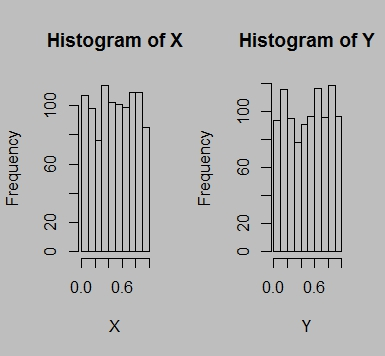
\includegraphics[scale=0.5]{fig1.jpeg}
      \caption{ Plot of Log Likelihood Function }
        \label{Figure 1}
\end{figure}

 
 \textbf {R Code}\\
 \begin{verbatim}
 install.packages("asbio")
 library(asbio)
 library(ElemStatLearn)
 library(MASS)

 X <- c(rep(0,7840), rep(1,1327), rep(2,239), 
         rep(3,42), rep(4, 14), rep(5,4), rep(6, 4), rep(7,1)) 
 n <- length(X) 
 negloglike<-function(lam) 
 { 
  sum(X) *log(lam) -n* lam + sum(log(factorial(X))) 
 }
  # Now we perform the optimization on the negative log like function. 
  out<-nlm(negloglike,p=c(0.5), hessian = TRUE) 
  #nlm is a nonlinear  minimization function
  mean(X)
  plot(negloglike)
\end{verbatim}

.\\
\textbf {Output : }\\
 The mean of x is 0.2151832\\
\begin{verbatim}
 > out
$minimum
[1] -47342038

$estimate
[1] 5000.5

$gradient
[1] -9470.592

$hessian
              [,1]
[1,] -8.143346e-05

$code
[1] 5

$iterations
[1] 5

To access the elements of out :
> out$estimate
[1] 5000.5
>  out$hessian
              [,1]
[1,] -8.143346e-05
\end{verbatim}





\item Finding the MLE of $ \lambda $ using computational methods\\

A likelihood for a statistical model is defined by the same formula as the density,
 but the roles of the data x and the parameter $ \theta $ are interchanged\\
${L_x}(\theta) = f_{\theta}(x).$ \\
The so-called method of maximum likelihood uses as an estimator of the unknown true parameter value,\\
 the point $ {\hat\theta_{x}}$ that maximizes the likelihood Lx.
This estimator is called the maximum likelihood estimator (MLE).
The R function nlm minimizes arbitrary functions written in R. \\
So to maximize the likelihood, we use the negative of the log likelihood in nlm.

\begin{verbatim}
 poisson.LL<-function(lam) sum(log(dpois(X,lam)))
 poisson.negloglik<-function(lam) -poisson.LL(lam) 
 nlm(poisson.negloglik,4,hessian=T)->out1
\end{verbatim}

\textbf {Output :}
\begin{verbatim}
> out1
$minimum
[1] 5508.31

$estimate
[1] 0.2151827

$gradient
[1] 0.0006020855

$hessian
         [,1]
[1,] 43972.98

$code
[1] 1

$iterations
[1] 11
\end{verbatim}


\item Estimating the probability that a randomly selected policy has 2 claims,\\
$ g(\lambda) = Pr (\lambda_{i} = 2) $ \\

$ \lambda = 0.215 $\\

$ Pr(\lambda_{i} = 2) = \dfrac{\lambda^{y}e^{-\lambda}}{y!} $\\\\

$ \rightarrow \dfrac{(0.215)^{2} e^{(-0.215)}}{2!} $\\ 

$ \rightarrow  {0.0186411} $\\\\


\end{enumerate}


\item Let ${X_{1}},....{X_{n}} \sim N(\theta , 1) $\\

 \begin{displaymath}
f(x) = \left\{
\begin{array}{lr}
1 & : x_i > 0 \\
0 & : x_i \leq 0
\end{array}
\right.
\end{displaymath}


\begin{enumerate}

\item Maximum Likelihood Estimator of $\theta$\\

$ f({x_i};\mu ,\sigma_{2}) = \dfrac{1}{\sigma \sqrt{2\pi}} exp{(- \dfrac{{{x_i}-\mu}^2}{2\sigma^{2}})}$\\\\

$ L[{\theta}] = \prod_{i=1}^{n} f({x_i})     $\\\\

$ = \prod_{i=1}^{n} \dfrac{1}{\sigma \sqrt{2\pi}} e^{-\frac{({x_i}-\mu)^{2}}{2 \sigma^{2}}} $\\\\

Since the $ \sigma $ = 1 \\

$ = \prod_{i=1}^{n} \dfrac{1}{ \sqrt{2\pi}} e^{-\frac{({x_i}-\theta)^{2}}{2 \sigma^{2}}} $\\\\

$ = 0 - \dfrac{2(\bar{X_{i}}-\theta)(-1)}{2} $ \\\\

$ ({x_i}-{\hat\theta}) \rightarrow 0$ (Setting the value to 0) \\\\

$  {\hat\theta_{MLE}} = \dfrac{\Sigma_{i=1}^{n} {X_i}}{n} = \bar X_{i} $\\\\


\item Maximum likelihood Estimator of $ \phi $ \\

Here we have Pr(${Y_1}$ = 1) = Pr(${X_1} >$ 0) = 1 - Pr$({X_1} \leq 0)$\\

So we have g$(\theta) = 1 -$ f(0)\\

$ \hat\phi_{MLE} = g ({\hat\phi_{MLE}}) $ \\

$ Pr(\theta,1)(X \geq 0) = Pr(\dfrac{X - \theta}{1} \leq \dfrac{0-\theta}{1})$\\

$ = 1 - Pr(Z \leq -\theta) $\\

Here Z is a standard normal distribution N(0,1)\\

$\rightarrow \hat\phi_{MLE} = 1 - \phi(-\theta)$\\

Note : The cdf of certain normal distribution cannot be calculated as you cant take the anti-deprivative of the normal distribution pdf.\\
So the function has to be made into a standard normal, which can be done using the pnorm function in R.\\ 
A certain probablity value  for a variable is obtained, but the actual cdf cannot be obtained.\\
It has to be experimentally calculated by converting the N($\theta$,1) distribution into a standard.\\


\item Computing the asymptotic error for $\theta$ and $\phi$\\

The Fischer information is a way of measuring the amount of information that an observable random variable X carries about an unknown parameter $\theta$ of a distribution that models X. \\

So we have, $I_{n}(\theta) = V(\theta) [\Sigma_{i=1}^{n} S(X_{i};\theta)]$\\

$\hat error = \sqrt{\dfrac{1}{-nE[\frac{d^2}{d\theta^2} log f (x|\theta)]}} $\\\\

$I_{n}(\theta) = -nE[\frac{d^2}{d\theta^2} log  (x|\theta)]$\\

On differentiating the above equation,\\

$ -nE[\dfrac{d}{d\theta}(x- \theta)]$\\

$-nE(-1) = nE $\\

So now the asymptotic error for $\theta$ is,\\

$ \rightarrow \sqrt{\dfrac{1}{n} }$\\

And now for the asymptotic error for $\phi$ \\

$\hat error = \left |g \prime (\hat \theta_{MLE})\right| [ \hat error(\hat \theta_{MLE})]$\\

$ g \prime (\hat \theta) = -\dfrac{1}{\sqrt{2\pi}} e^{\frac{{\theta - \mu}^2}{2}}$\\\\

$= \left| \dfrac{1}{\sqrt{2\pi}} e^{\frac{{(-\theta)}^2}{2}} \right |$\\\\

$ \rightarrow \left| \dfrac{1}{\sqrt{2\pi}} e^{\frac{{(-\theta)}^2}{2}}\right | \sqrt{\dfrac{1}{n}}$\\\\

So now substitute $\theta$ = x;\\

$ \rightarrow \left | \dfrac{1}{\sqrt{2\pi}} e^{\frac{{(-x)}^2}{2}}\right | \sqrt{\dfrac{x}{n}}$\\\\







\end{enumerate}


\item Consider the given data\\
 ${X_1}$,${ X_2}$, ${X_3}$, . . . ${X_n}$,\\
$ {Y_1}$, ${Y_2}$, . . .${ Y_m}$\\
 where the X′s come from model f andthe Y′s come from model g.\\
 
 All X′s are independent and all Y′s are independent and any X is independent from any Y .\\\\

 
 Now f(x) = $\dfrac{1}{\theta} e^{({-\frac{x}{\theta}})}$ for x $>$ 0 and \\
 
 g(y) = $ e^{({-\frac{5y}{\theta}})}({1 - e^{({−\frac{5}{\theta})}}})^{(1-y)}$ where y is either 0 or 1.\\
 

 
 \begin{enumerate}

\item
The Joint Distribution $\rightarrow$ f(x).g(x) \\\\

$(\dfrac{1}{\theta} e^{({-\frac{x}{\theta}})})$ * $( e^{({-\frac{5y}{\theta}})}({1 - e^{({−\frac{5}{\theta})}}})^{(1-y)})$\\

$f_{x,y} (X,Y) = \dfrac{1}{\theta} e^{\dfrac{-x-5y}{\theta}} ({1 - e^{-\frac{5}{\theta}}})^{(1-y)}$\\\\

$ L(\theta) = \prod_{i=1}^{n}(\dfrac{1}{\theta}e^{\dfrac{-x-5y}{\theta}}({1 - e^{-\frac{5}{\theta}}})^{(1-y)})$\\\\

$\left(\theta\right)=\frac{1}{\theta ^{n_1}} \left(e^{-\sum_{i=1}^{n_1}\frac {x_i}{\theta}}\right)\left(e^{-5\sum_{i=1}^{n_2}\frac {y_i}{\theta}}\left(1-e^{\frac{-5}{\theta}}\right)^{\left(n_2-\sum_{i=1}^{n_2}y_2\right)}\right)$\\\\


\item
Now we have 10 observations from f - 2.8, 5.6, 24.7, 6.5, 1.6, 10.6, 1.0, 7.8, 7.2,13.9 
and 15 observations from g: 0, 0, 0, 1, 1, 1, 0, 0, 1, 0, 0, 0, 0, 0, 0. 
Now to compute the MLE for θ.\\\\

\begin{verbatim}
 x <- c(2.8,5.6,24.7,6.5,1.6,10.6,1.0,7.8,7.2,13.9)
 nx <- length(x)
 y <- c(0,0,0,1,1,1,0,0,1,0,0,0,0,0,0)
 ny <- length(y)
 mlefunc <- function(theta)
 {
  -nx * log(theta) - sum(x)/theta - 5 * sum(y)/theta +
                         (ny-sum(y)) * log(1-exp(-5/theta))
  }
opt <- optimize(func1, interval=c(0,10),maximum=TRUE)
\end{verbatim}




\textbf {Output :}\\
\\The maximum Likelihood estimator for $\theta$ is estimated to be 5.971734\\

\end{enumerate}

\end{enumerate}
\end{document}